
\documentclass[12pt]{article}
\usepackage{geometry}
\geometry{a4paper}


\usepackage{color}
\usepackage{hyperref}
\usepackage{amsmath}
\usepackage{amsfonts}
\usepackage{amssymb}
\usepackage{graphicx}
\usepackage{tcolorbox}
\usepackage{listings}
\usepackage{here}
\usepackage{txfonts}
\usepackage{algorithm}
\usepackage{algorithmic}
\usepackage{siunitx}
\usepackage{xcolor}
\usepackage{ascmac}
%\usepackage{fancybx}

\lstset {language = c++,
  basicstyle = \ttfamily \scriptsize,
  commentstyle = \textit,
  frame = tRBl,
  framesep = 5pt,
  showstringspaces = false,
  numbers = left,
  stepnumber = 1,
  numberstyle = \tiny,
  tabsize = 2,
  keywordstyle = \bfseries \color{blue},
  stringstyle=\color{magenta},
  commentstyle=\color{red},
  morecomment=[l][\color{red}]{\#}
  showstringspaces=false, % don't mark spaces in strings
}
\newcommand{\bi}[1]{\mathbf{#1}}
\newcommand{\bs}[1]{\boldsymbol{#1}}  % bold for greek characters
\newcommand{\bbR}{\mathbb{R}}

\author{Nobuyuki Umetani}


%%%%%%%%%%%%%%%%%%%%%%%%%%%%%%%%%

\title{Finite Elemnet Method:\\Helmholtz Equation \footnote{This is just a memorandum not to forget what I learned when I was a master student.}}

\author{Nobuyuki Umetani}

\begin{document}

\maketitle
\tableofcontents


\section{Introduction}
In this document, we explain how we can numerically solve acoustic equations using the Finite Element Method (FEM).

Sound is a pressure wave that propagates inside space.




\paragraph{Why PDE?}
Since equation is about the spatial distribution of the pressure, we need to describe how the sound propagate using a Partial Differential Equation (PDE).
%
There are two types of the PDE for sound both very useful for different context.
%
The one is the Wave Equation and the other is Helmholtz equation.
%
We will explain the difference between equations later.
%


\paragraph{How to solve PDE?}
Once we describe the PDE, we can solve it using a numerically for a given shape.
%
There are Finite Difference Method (FDM), Finite Element Method (FEM), and Finite Boundary Method (FBM).
%



For simplicity, let's assume that the sound is made out of a sin wave with a constant frequency.


\paragraph{Two ways to interpret wave propagation}
If you look only how the crest and thorough travel trough the air, the wave looks like it is constantly moving.
the wave looks like transient behavior.
%
However, the pressure is always changing in the sin wave.
%
In the `` phase space '
%
The complex number is very good at representing harmonically oscillating value in one single variable
%
\begin{equation}
e^{i \theta} = \sin \theta + i \cos \theta
\end{equation}



%
There are two ways to model the

The document is largely based on a book: \cite{ihlenburg 1998 finite}



\section{Wave Equation}

single mass and spring.
%
mass spring connected together.
%
mass try to go back original undeformed state by pushing the neighbor.
%
The force propagates.

\paragraph{Two types of waves}
There are two types of waves: transversal wave (sheer wave) and density wave.
%
Good example of these two waves are the waves of earthquake.
%
Born and grow in Japan, I know from experience there are two kind of vibration P-wave and S-wave.
%
P-wave comes faster than the S-wave.
%
%
So the force is normal direction of the region. There is no sheer force.
%
The sound propagates as density waves.
%




\subsection{Relationship between Pressure and Density: from the Mass Conservation Law}

The mass conservation law basically says the mass does not disappear or appearance.
%
\begin{tcolorbox}[title=Mass Conservation Law]
\begin{eqnarray}
&&\frac{D \rho}{D t} = 0 \\
&\Leftrightarrow& \frac{\partial\rho}{\partial t} + \nabla\cdot(\rho\bi{v}) = 0
\label{eqn:mass_conservation}
\end{eqnarray}
\end{tcolorbox}
%
This equation says at the given a region $\Omega$ that \ textit {moves together} with the air with the velocity $\bi{v}$, the weight of the air inside the $m$ does not change.
%

equation of motion of the compressive fluid can be written as
\begin{tcolorbox}[title=Compressive Navier - Stokes Equation]
\begin{equation}
\frac{\partial (\rho \bi{v})}{\partial t} + \bi{v}\cdot\{\nabla \otimes (\rho \bi{v})\} = -\nabla p + \nabla\cdot\bi{T}
\label{eqn:compressive_fluid}
\end{equation}
\end{tcolorbox}


Here, $\bi{T}$ is the Cauchy stress tenor that encode force inside the flow arise from the deformation of the fluid (eg, viscosity).


\paragraph{Sound component of the velocity}
We ignore the advection term and the viscosity term which is second term in the LHS and and the second term of the RHS.
%
This simplification is simply possible due to the time averaged velocity $\bi{v}$ is very slow compared to the speed of sound.

Thus, the velocity of the
%
The \eqref{eqn:compressive_fluid} can be written as as:
%
\begin{equation}
\frac{\partial (\rho \bi{v})}{\partial t} = -\nabla p
\label{eqn:simple_compressive_fluid}
\end{equation}
%

Let's take the divergence to the both sides of the~\eqref{eqn:simple_compressive_fluid}
%
\begin{eqnarray}
&& \nabla\cdot\frac{\partial (\rho \bi{v})}{\partial t} =-\nabla\cdot(\nabla p)\\
&\Leftrightarrow& \frac{\partial}{\partial t}\{\nabla\cdot(\rho\bi{v})\} = -\nabla\cdot(\nabla p)\\
&\Leftrightarrow& \frac{\partial^2 \rho}{\partial t^2} = -\nabla\cdot(\nabla p)
\end{eqnarray}


\subsection{Relationship between pressure and density: from the Gas Equation}
%
Ideal gas equation has:
\begin{equation}
p_0=\rho_0 RT_0
\end{equation}
%
where $R$ is a coefficient (for simplicity, $R$ is not the one using the moll number).
%
Yet, $p_0$, $\rho_0$ and $T_0$ is reference pressure, reference density and reference temperature.
%
Here we assume no heat diffusion. Isothermal compression has
%
\begin{equation}
p = \rho^\gamma RT_0
\end{equation}
%
where $\gamma$ is the \textit{heat capacity ratio} ~ (specific heat ratio)

%
Let's examine the relationship density and the pressure under the small fluctuation from the reference state.
%
\begin{equation}
\left.\frac{\partial p}{\partial \rho}\right|_{\rho_0} = \gamma \rho^{\gamma-1}_0 RT_0 =\frac{\gamma\rho^{\gamma}_0 RT_0}{\rho_0} = \frac{\gamma p_0}{\rho_0} = \frac{\gamma\rho_0 RT_0}{\rho_0} = \gamma RT_0
\label{eqn:pressure_density_flucturation}
\end{equation}



\subsection{the Wave Equation}
%
Now we have two equations for two variables (pressure and density), meaning that we can erase one variable to make it one one with with one variable.
%
From the Equation ~ \eqref{eqn: pressure_density_flucturation}, the small perturbation of density $d\rho$and the pressure $dp$ have the relationship:
%
\begin{equation}
d\rho = \frac{1}{\gamma RT_0} dp
\end{equation}

Assuming this small perturbation is result from the small change of density and pressure over time, we have
%
\begin{equation}
\frac{\partial^2 \rho}{\partial t^2} = \frac{1}{\gamma RT_0} \frac{\partial^2 p}{\partial t^2}
\end{equation}
%
\begin{equation}
\frac{\partial^2 p}{\partial t^2} = -(\gamma RT_0) \nabla\cdot(\nabla p)
\end{equation}

This is the wave equation for the pressure.
%
The speed of the sound $c$ can be written as:
\begin{equation}
c = \sqrt{\gamma RT_0 }
\end{equation}




\begin{tcolorbox}[title=Wave Equation]
\begin{equation}
\nabla\cdot(\nabla U) - \frac{1}{c^2} \frac{\partial^2 U}{\partial t^2} =  0
\label{eqn:wave_equation}
\end{equation}
\end{tcolorbox}


\section{Helmholtz Equation (Helmholtz equation)}

Here we transform the Wave Equation \eqref{eqn:wave_equation} into the Helmholtz equation.

\subsection{Separation of Variables to Derive Helmhotlz Equatoin}

We assume that the solution $U$ is the multiple of harmonic vibration part and spatial distribution part.
%
Here the field is vibration with the \textit{angular frequency} ~ $\omega$ and the spatial distribution $u(\bi{x})\in\mathbb{C}$.

\begin{equation}
U(\bi{x},t) = u(\bi{x}) e^{i\omega t}
\end{equation}

Substituting this into the following equation

\begin{equation}
 \nabla\cdot(\nabla u) e^{i\omega t} - \frac{1}{c^2} (-\omega^2) u e^{i\omega t}= 0
\end{equation}

. It satisfies the following Helmholtz equation.
\begin{tcolorbox}[title=Helmholtz Equation]
\begin{equation}
\nabla\cdot(\nabla u) + k^2 u = 0
\end{equation}
\end{tcolorbox}
where $k=\frac{\omega}{c}$ is the wave number (wave number).



\subsection{Kernel Function}
Let's consider the Helmholtz equation with the delta function as follows on the right hand side.

\begin{equation}
\nabla\cdot(\nabla u) + k^2 u = \delta(r)
\end{equation}


\begin{equation}
r=|x|
\end{equation}

Since the right side is point symmetric, the solution also becomes point symmetric. Since there are kernel numbers, simulation using the boundary element method (BEM) is also possible.
The solution is different for 2D and 3D, and it is as follows.

\subsubsection{Two-dimensional time}

In the case of two dimensions, or in the case of axisymmetric problem, analytical solution can be written with first kind Hankel function as follows.

% \ begin {itembox} {analytical solution in the case of two dimensions}
\begin{equation}
g(r)=\frac{iH^{(1)}_0(kr)}{4}
\end{equation}
% \ end {itembox}

The Hankel function that comes out here is the sum of the first kind Bessel function $J_0$ and the second kind Bessel function $Y_0$ multiplied by a complex unit as follows.

\begin{equation}
H^{(1)}_0 = J_0 + iY_0
\end{equation}

The Bessel function of the analytical solution is described in more detail below.
Bessel function http://ums.futene.net/wiki/Math/bessel/index.html

\subsubsection{three dimensional time}

In the case of three dimensions, the analytical solution can be written with the first kind Hankel function as follows.

% \ begin {itembox} {Analysis solution in three dimensions}
\begin{equation}
g(r)=\frac{e^{ikr}}{4\pi r}
\end{equation}
% \ end {itembox}



\section{Boundary Condition}

\subsection{Total reflection boundary condition (Hard wall)}

Let's consider that the waves are completely reflected at the boundary. That is, assuming that the boundary is the x = 0 plane, the normal vector of the boundary condition is taken as the x axis, and the component in contact with the boundary of the wave vector is taken as the y axis.

\begin{figure}[htbp!]
\center
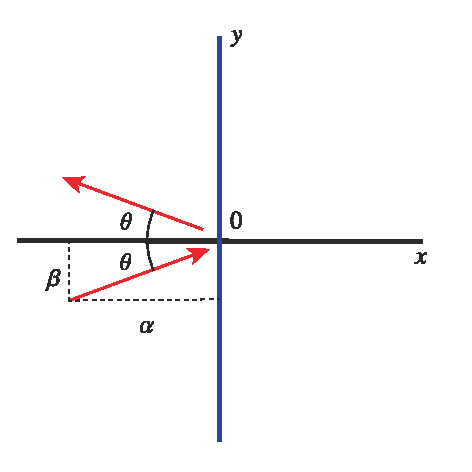
\includegraphics[width=80mm]{images/ref_boundary.pdf}
\caption{relationship between boundary and wevenumber vector}
\end{figure}

At this time, the spatial distribution of the sound pressure is expressed by the following equation.

\begin{equation}
p(x,y,z)=\bar{p}e^{i(\alpha x+\beta y)} + \bar{p} e^{i(-\alpha x+\beta y)}
\end{equation}

Consider the differentiation in the normal direction of the sound field.

\begin{eqnarray}
\left.\frac{\partial p}{\partial x}\right|_0
&=& \bar{p}i\alpha e^{i(\alpha x+\beta y)} - \bar{p}i\alpha e^{i(-\alpha x+\beta y)}\\
&=& \bar{p}i\alpha e^{i\beta y}\left(\;e^{i\alpha x} - e^{i\alpha x}\right)\\
&=& \bar{p}i\alpha e^{i\beta y}\left(1-1\right) \\
&=& 0
\end{eqnarray}

When the coordinate system is returned to a general thing, it becomes as follows.

\begin{tcolorbox}[title=boundary condition (total reflection)]
\begin{equation}
\frac{\partial p}{\partial n}= 0
\end{equation}
\end{tcolorbox}







\subsection{Absorbing Boundary Condition}
Let's consider a wave passing through without reflecting the boundary. Let the boundary be the x = 0 plane, take the normal vector of the boundary condition to the x axis and the component touching the boundary of the wave vector to the y axis.


\begin{figure}
\center
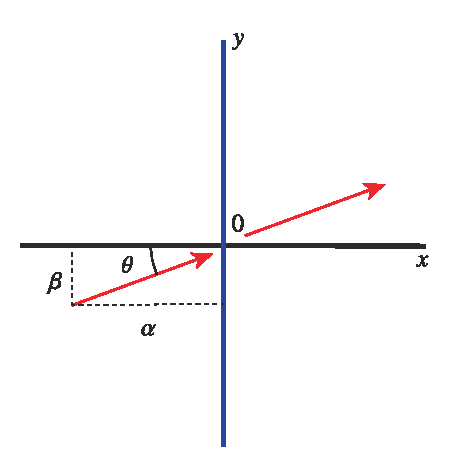
\includegraphics[width=80mm]{images/abc_boundary.pdf}
\caption{Positional relationship between boundary and wavenumber vector}
\end{figure}




At this time, the sound pressure is expressed by the following equation.

\begin{equation}
p(x,y,z)=\bar{p}e^{i(\alpha x+\beta y)}
\end{equation}


\begin{equation}
k = \sqrt{\alpha^2+\beta^2},\;\;\; \theta = \tan^{-1}\left(\frac{\beta}{\alpha}\right)
\end{equation}


\begin{equation}
\sigma=\sin\theta = \frac{\beta}{k},\;\;\;\alpha = k\cos\theta = k\sqrt{1-\sigma^2}
\end{equation}


\begin{equation}
\frac{\partial p}{\partial y} = i\beta p\;\;\;\Leftrightarrow\;\;\; \frac{\partial^2 p}{\partial y^2} = i\beta\frac{\partial p}{\partial y}=-\beta^2p \;\;\;\Leftrightarrow\;\;\; \beta^2 = -\frac{1}{p}\frac{\partial^2 p}{\partial y^2}
\end{equation}


\begin{eqnarray}
\frac{\partial p}{\partial x} &=& i\alpha p = i k \left(\sqrt{1-\sigma^2}\right)p \\
&\simeq& ik\left(1-\frac{\sigma^2}{2}\right)p = ik\left(1+\frac{\beta^2}{2k^2}\right)p = \left(ik+\frac{i}{2k}\frac{\partial^2 }{\partial y^2}\right)p
\end{eqnarray}

Because it is $\frac{\partial p}{\partial z}=0$,

\begin{equation}
\frac{\partial p}{\partial x} \simeq  \{ik+\frac{i}{2k}\left(\frac{\partial^2}{\partial y^2}+\frac{\partial^2}{\partial z^2}\right)\}p
\end{equation}

. In the above equation, the normal vector is taken on the x axis and the component in contact with the boundary of the wave vector is taken on the y axis. This is normalized to the normal $n$ and its directional derivative in contact therewith as follows.

\begin{equation}
\frac{\partial p}{\partial n} \simeq \left(ik+\frac{i}{2k}\Delta_t\right)p
\end{equation}

However, $\Delta_t$ is a Laplacian in the tangent plane. In the numerical analysis, the absorption boundary condition is expressed by using the above approximate expression.

\begin{tcolorbox}[title=absorption boudnary condition]
\begin{equation}
\frac{\partial p}{\partial n} = \left(ik+\frac{i}{2k}\Delta_t\right)p
\end{equation}
\end{tcolorbox}

{\bf If the wavenumber vector has a large angle with respect to the boundary normals, the error of this approximation becomes large.} For a more accurate approximation, a more complicated and higher order derivative is required, and here Absent.



\subsection{Sound emission from solid}
If the solid oscillates periodically with angular velocity $w$, the solid velocity $\bi{v}_s$

\begin{equation}
\bi{v}_s = \bar{\bi{v}}e^{iwt}.
\end{equation}

At this time, assuming that viscosity is neglected, the normal direction component of the velocity of the fluid coincides with the normal direction velocity of the solid, so the following is obtained.

\begin{equation}
\bi{v}_f\cdot\bi{n} = \bar{\bi{v}}\cdot\bi{n}e^{iwt}
\end{equation}

Assuming that the pressure changes periodically according to the speed change of the fluid, it is as follows.

\begin{equation}
 p = \bar{p} e^{iwt}
\end{equation}

This is the Navier-Stokes equation ignoring advection and viscosity

\begin{equation}
\frac{\partial (\rho \bi{v})}{\partial t} = -\nabla p
\end{equation}

Substitute into $\bi{n}$ and calculate the inner product of $\bi{n}$ as follows

\begin{equation}
\rho iw\bar{\bi{v}}\cdot\bi{n} = - (\nabla \bar{p}\cdot\bi{n})
\end{equation}

Is satisfied.

\begin{equation}
\frac{\partial p}{\partial n} = -\rho iw(\bar{\bi{v}}\cdot\bi{n})
\end{equation}




\section{Finite Element Discretization}

\subsection{Weak form of the Helmholtz Equation}

Let's weakly formulate the following expression.

\begin{equation}
 -\{\nabla\cdot(\nabla p)+k^2 p\} = f
\end{equation}

We multiply $\delta p$ to the both hand side and integrate over the domain $V$.
%
\begin{equation}
\int_V -\delta p \{\nabla\cdot(\nabla p) + k^2 p \} dV = \int_V \delta p f dV\;\;\;\forall \delta p
\end{equation}
%
When applying the Green-Gauss theorem to the first term of the above equation,

\begin{eqnarray}
\int_S -n\cdot (\delta p\nabla p) dS + \int_V \nabla\delta p \cdot\nabla p -  \delta p k^2 p  dV &=& \int_V \delta p f dV\forall \delta p\\
\Leftrightarrow \int_S -\delta p\frac{\partial p}{\partial n} dS + \int_V \nabla\delta p \cdot\nabla p -  \delta p k^2 p  dV &=& \int_V \delta p f dV\;\;\;\forall \delta p
\end{eqnarray}

\begin{tcolorbox}[title=Weak Formulation of the Helmholtz Equation]
\begin{equation}
\int_V \nabla\delta p \cdot\nabla p - \delta p k^2 p  dV = \int_V \delta p f dV + \int_S \delta p\frac{\partial p}{\partial n} dS \;\;\;\forall \delta p
\end{equation}
\end{tcolorbox}


\subsection{FEM Discretizatio of the Helmholtz Equation (finite element method discretization of Helmholtz equation)}

Discretize only the term contributing to volume integration (terms related to surface area can be added later). If the mesh is divided, the volume can be represented by the sum of each element.

\begin{equation}
\sum_e\int_{V_e} \nabla\delta p \cdot\nabla p -  \delta p k^2 p  dv = \sum_e\int_{V_e} \delta p f dv\;\;\;\forall \delta p
\end{equation}

Suppose that interpolation is performed as follows using the interpolation function $N$ in the element.

\begin{equation}
\delta p = N^p \delta p^p\;\;\;\; p = N^q p^q
\end{equation}

By substituting the interpolation equation of the interpolation function into the above equation and transforming the equation, simultaneous linear equations are obtained.

\begin{eqnarray}
&&\sum_e\int_{V_e} \nabla(N^p\delta p^p) \cdot\nabla (N^q p^q) -  k^2(N^p\delta p^p) (N^q p^q)  dV = \sum_e\int_{V_e} (N^p\delta p^p) f dV\;\;\;\forall \delta p\\
&\Leftrightarrow& \sum_e \delta p^p \left[\int_{V_e} \nabla N^p \cdot\nabla N^q -  k^2N^pN^qdV\right] p^q  = \sum_e\delta p^p\int_{V_e} N^p f dV\;\;\;\forall \delta p\\
&\Leftrightarrow& \sum_e \left(\delta p^p A_e^{pq} p^q \right) = \sum_e\left(\delta p^p f^p\right)\;\;\;\forall \delta p\\
&\Leftrightarrow& \delta p^a\left(\sum_e A_e^{pq}\right) p^b = \delta p^a \left(\sum_ef^p\right)\;\;\;\forall \delta p^a\\
&\Leftrightarrow& A^{ab}\ p^b = F^a
\end{eqnarray}

However, it is assumed that the numbering of the nodes within the element $\{p,q\}$ corresponds to the numbering of the whole node $\{a,b\}$.
It can be seen that the element stiffness matrix is ​​as follows.


\begin{tcolorbox}[title=Element Stiffness Matrix (element stiffness matrix)]
\begin{equation}
A_e^{pq} = \int_{V_e} \nabla N^p \cdot\nabla N^q -  k^2N^pN^qdV
\end{equation}
\end{tcolorbox}


\subsection{weak formalization of absorption boundary condition and discretization of finite element method}

\subsubsection{Weak Formulation}

Integral expression of boundary

\begin{equation}
\int_S \delta p \frac{\partial p}{\partial n} dS
\end{equation}

Expression of boundary condition

\begin{equation}
\frac{\partial p}{\partial n} = \left(ik+\frac{i}{2k}\Delta_t\right)p
\end{equation}

Substitute

\begin{equation}
\int_S \delta p \left(ik+\frac{i}{2k}\Delta_t\right)p ds = \int_S \delta p (ik p)-\frac{i}{2k}(\nabla_t\delta p)\cdot(\nabla_t p) ds +  \int_{\partial S}\frac{i}{2k}\delta p \frac{\partial p}{\partial n_t} dt
\end{equation}

In the following discussion, we ignore the third term on the right side as $\partial S = \emptyset$ for simplicity.


\subsubsection{Finite Element Discretization}
Assuming that the surface is meshed, the integral can be expressed by the sum of each element.

\begin{equation}
\int_S \delta p (ik p)-\frac{i}{2k}(\nabla_t\delta p)\cdot(\nabla_t p) dS = \sum_e \int_{S_e} \delta p (ik p)-\frac{i}{2k}(\nabla_t\delta p)\cdot(\nabla_t p) dS
\end{equation}

Assume that interpolation is performed as follows using the interpolation function $N$ within the surface element.

\begin{equation}
\delta p = N^p \delta p^p\;\;\;\; p = N^q p^q
\end{equation}

Substituting this for the above gives the element stiffness matrix at the boundary.

\begin{equation}
A^{pq}_e = \int_{S_e} ik N^p N^q -\frac{i}{2k}(\nabla N^p)\cdot(\nabla N^q) dS
\end{equation}

\subsubsection{Comparison of Accuracy by Order of Absorption Boundary Condition}
Depending on the accuracy of the absorption boundary condition, it is confirmed by the following two formulas how much the solution changes. Equation (1) is the first order absorption boundary condition, and equation (2) is the second order absorption boundary condition.

\begin{eqnarray}
\begin{array}{ll}\frac{\partial p}{\partial n} = ikp & \;\;\;\cdots\;\;\; (1)\\  \frac{\partial p}{\partial n} = \left(ik+\frac{i}{2k}\frac{\partial^2 }{\partial y^2}\right)p & \;\;\;\cdots\;\;\; (2)\end{array}
\end{eqnarray}

The real part of the solution is indicated by a contour when using the equation (1) on the left figure of Figure 3 and the equation (2) as the boundary condition on the right figure.


\begin{figure}[htbp]
\begin{center}
 \begin{minipage}{0.45\hsize}
  \begin{center}
   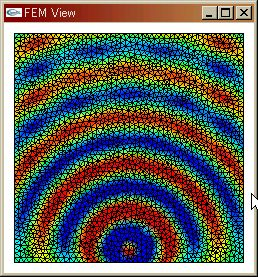
\includegraphics[bb=0 0 300 300,width=5cm]{images/abc_bound_1st.jpg}
  \end{center}
  \caption{first order absorption boudanry condition}
  \label{fig:abc_bound_1st}
 \end{minipage}
 \begin{minipage}{0.45\hsize}
  \begin{center}
   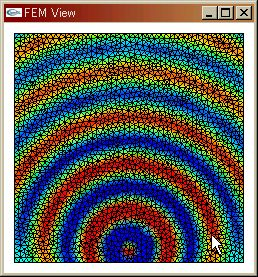
\includegraphics[bb=0 0 300 300,width=5cm]{images/abc_bound_2nd.jpg}
  \end{center}
  \caption{second order absorption boundary condition}
  \label{fig:abc_bound_2nd}
 \end{minipage}
\end{center}
\end{figure}


It can be seen that neither the primary nor secondary has a point symmetry from the wave source. This is because radiation boundary conditions are still not perfect and there is wall influence. Since the low-order radial boundary condition is based on the assumption that the boundary and the wave traveling direction are nearly perpendicular, when the wave traveling direction and the boundary are close to parallel as shown in the lower part of the screen, an error appears. Nonetheless, it turns out that the secondary is improved as compared with 1. In the first order, the interference pattern between the wall and the reflected wave can be seen on the upper side of the screen, but almost no interference pattern is seen in the second order.









\section{Solving Linear System form Discretized Helmholtz Equation using Iterative Method}
It is the iterative solution that solves the sparse matrix like the finite element method most efficiently, but it is difficult because the coefficient matrix is ​​non-Hermitian and indefinite value
Considering the absorption boundary condition and viscosity, the coefficient matrix obtained by the finite element method discretization is a complex matrix. This matrix is ​​symmetric, but not Hermitian, so you can not use a method like the CG method. We solve the matrix using the BiCG method (COCG \ cite {9 - cocg} in the case of complex number), CGNR method, BiCGStab method, GMRes method extended to complex number, as used in real asymmetric matrix.

\subsection{COCG Algorithm}
The Conjugate orthogonal-conjugate gradient (COCG) method is a special case in the case of a complex number of the BiCG method, in which the shadow vector of the BiCG method is a conjugate vector. The algorithm of the COCG method is as follows.

\subsubsection{Algorithm (COCG method)}

\begin{enumerate}
\item $Compute$ $\bi{r}_0=\bi{b}-\bi{A}\bi{x}_0$
\item $Set$, $\bi{p}_0=\bi{r}_0$
\item $For$ $k=0,1,\ldots,m\quad$$Do:$
\item $\;\;\; \alpha_k=\frac{(\bar{\bi{r}}_k,\bi{r})}{(\bar{\bi{A}\bi{p}}_k,\bi{p}_k)}$
\item $\;\;\; \bi{x}_{k+1}=\bi{x}_k+\alpha_k\bi{p}_k$
\item $\;\;\; \bi{r}_{k+1}=\bi{r}_k-\alpha_k\bi{A}\bi{p}_k$
\item $\;\;\; \beta_k=\frac{\bar{(\bi{r}}_{k+1},\bi{r}_{k+1})}{(\bar{\bi{r}}_,\bi{r}_k)}$
\item $\;\;\; \bi{p}_{k+1}=\bi{r}_{k+1}+\beta_k\bi{p}_k$
\item $End \quad Do$
\end{enumerate}

The symbol $(\;,\;)$ here represents the inner product of complex numbers. That is, it is $(a,b)=\bar{\bi{a}}^T\bi{b}$. For the Hermitian matrix, we will use this inner product in the algorithm when applying the CG method, but note that in the COCG method, instead of the inner product, we add the multiplication of the components $(\bar{a},b)=\bi{a}^T\bi{b}$.

\subsection{Precondiotner}

In addition, since the coefficient matrix obtained when discretizing Helmholtz with large wavenumber is unknown, a special pretreatment method (complex shift Laplace preprocessing) may be used to stably solve by the COCG method or the BiCGStab method . For details, please refer to \ cite {erlangga2004class} \ cite {vuik} \ cite {erlangga2005robust}.

\section{Formulation for Axisymmetric Problem}
As shown in the following figure, consider the axisymmetric three-dimensional problem, that is, when all shapes, boundary conditions, and physical property values ​​are axisymmetric, the solution is also axisymmetric. In this case, it can be reduced to a two-dimensional problem in the cross section and the cost of three-dimensional analysis can be greatly reduced.

\begin{figure}[tbp]
\begin{center}
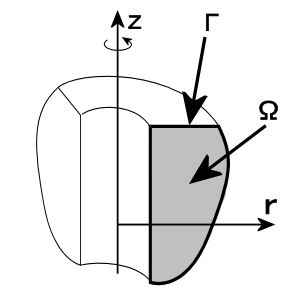
\includegraphics[bb=0 0 100 100,width=5cm]{images/cylinder_domain.jpg}
\caption{axis symmetric region}
\end{center}
\end{figure}


\subsection{Weak Formulation}
In the case of the axisymmetric case, the Helmholtz equation is discretized two-dimensionally about the cross section by the finite element method. The weak form of the Helmholtz equation was as follows.

\begin{equation}
\int_V \nabla\delta p \cdot\nabla p - \delta p k^2 p  dV = \int_V \delta p f dV + \int_S \delta p\frac{\partial p}{\partial n} dS \;\;\;\forall \delta p
\end{equation}

Let's convert the integral variable to $\{x,y,z\}\rightarrow \{r,\theta,z\}$ as follows.

\begin{eqnarray}
\left\{\begin{array}{l}
x\rightarrow rsin\theta\\
y\rightarrow rcos\theta\\
z\rightarrow z\end{array}\right.
\end{eqnarray}

The absolute value of Jacobian in this case is

\begin{eqnarray}
\det J(r,\theta,z)=\det \left[\begin{array}{lll}
\sin\theta & r \cos\theta & 0 \\
\cos\theta & -r\sin\theta & 0 \\
0 & 0 &  1
\end{array}\right] = r
\end{eqnarray}

Therefore, it becomes $dxdydz = r drd\theta dz$. Also, as shown in the figure below,
axis surface.jpg

\begin{equation}
dS = rdsd \theta
\end{equation}

If this is substituted above,

\begin{equation}
\int_\theta\int_r\int_z r\nabla\delta p \cdot\nabla p - r\delta p k^2 p  dzdrd\theta = \int_\theta\int_r\int_z \delta p f rdzdrd\theta + \int_\theta \int_s \delta p\frac{\partial p}{\partial n} rdsd\theta\;\;\;\forall \delta p
\end{equation}

Since the integrand does not change in the $\theta$ direction, we can remove the integral of $\theta$. Also, if we write $v$ for the two-dimensional integral region of the cross section and $s$ for the cross section boundary, weak formalization for the axisymmetric problem as shown below is obtained.

\begin{tcolorbox}[title=weak form of the Helmholtz equation on the axisymmetric problem]
\begin{equation}
\int_r\int_z r\nabla\delta p \cdot\nabla p - r\delta p k^2 p  dzdr = \int_r\int_z \delta p f rdzdr + \int_s \delta p\frac{\partial p}{\partial n} rds\;\;\;\forall \delta p
\end{equation}
\end{tcolorbox}


\subsection{Finite Element Discretiazation}
Assuming that the two-dimensional area $v$ of the cross section is divided into meshes, the integral of the above equation can be obtained by adding all the integration within each element. In other words,

\begin{equation}
\int_{v_e} r\nabla\delta p \cdot\nabla p - r\delta p k^2 p  dv = \int_{v_e} \delta p f rdv + \int_{s_e} \delta p\frac{\partial p}{\partial n} rds\;\;\;\forall \delta p
\end{equation}

Here, {\ bf calculate 1 term and 2 term related to volume integration}. , Let us say that $T$ and $\delta T$ are discretized using the interpolation function $N$ in the element, assuming that the variation is performed by the Galerkin method as follows.
$p = N^q p^q$, $\delta p = N^p \delta p^p$
Substituting these into weak form, we can derive the element stiffness matrix, the overall stiffness matrix as follows. However, in formula deformation it is assumed that the numbering $\{p,q\}\rightarrow \{a,b\}$ in the element holds.

\subsubsection{First Term Left Hand Side}

\begin{eqnarray}
&& \sum_e\int_{v_e} r\nabla N^p\delta p^p\nabla N^qp^q - rk^2N^p\delta p^pN^q p^qdv\\
&\Leftrightarrow& \sum_e\left(\delta p^p\int_{v_e}  r\nabla N^p\nabla N^q - rk^2 N^pN^qdv p^q\right)\\
&\Leftrightarrow& \delta p^a\left(\sum_e A_e^{pq} \right) p^b\\
&\Leftrightarrow& \delta p^a A^{ab} p^b
\end{eqnarray}

\begin{tcolorbox}[title=coefficient matrix]
\begin{equation}
A_e^{pq}=\int_{v_e}r\nabla N^p\nabla N^q - rk^2 N^pN^q dV
\end{equation}
\end{tcolorbox}


\subsubsection{First Term Right Hand Side}

\begin{eqnarray}
&& \sum_e\int_{v_e} \delta p f rdv\\
&\Leftrightarrow& \sum_e\left(\delta p^p\int_{v_e}r N^p f dv\right)\\
&\Leftrightarrow& \delta p^a\left(\sum_e F^p_e \right)\\
&\Leftrightarrow& \delta p^a F^a
\end{eqnarray}

It can be seen that these are obtained by adding together the following matrices in element units.

\begin{tcolorbox}[title=external force vector]
\begin{equation}
F_e^p = \int_{V_e} rN^p f dv
\end{equation}
\end{tcolorbox}

\subsection{Example of finding open end correction}
In order to verify the analysis accuracy of the Helmhltz equation of the axisymmetric problem, we conducted an experiment to obtain open end correction. Open end correction means that resonance occurs at a place where the wavelength is slightly longer than the resonant wavelength calculated as an integral multiple of the length of the pipe or the like when considering the resonance of the pipe . If one end is opened like a pipe, the air around it will also vibrate together, so we need to consider the effect.

\begin{figure}[tbp]
\begin{center}
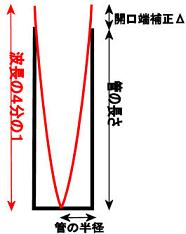
\includegraphics[bb=0 0 150 150,width=5cm]{images/open_end_modify.jpg}
\caption{open end correction}
\end{center}
\end{figure}



The setting of the numerical experiment is as follows, assuming that it is an axisymmetric problem, a mesh is cut in the area of ​​the air around the pipe and the opening.


\begin{figure}[tbp]
\begin{center}
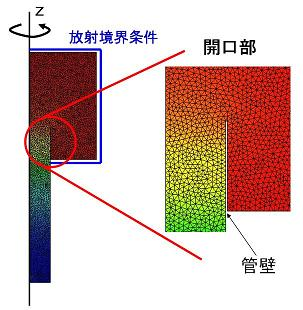
\includegraphics[bb=0 0 200 200,width=5cm]{images/fem_analysis_condition.jpg}
\caption{FEM solution}
\end{center}
\end{figure}


Find the resonance frequency of this tube and determine the open end correction from its wavelength and tube length. When determining the resonance frequency, place the point sound source at an arbitrary place (the bottom of the tube in this experiment) and monitor how much the sound emitted from the sound source amplifies while changing the frequency, and the amplification factor peaks , The resonance frequency was taken as the frequency.
The theoretical value of open end correction Δ is Δ = 0.61 ... × radius and is determined as \ cite {levy}, which is the graph below.


\begin{figure}[tbp]
\begin{center}
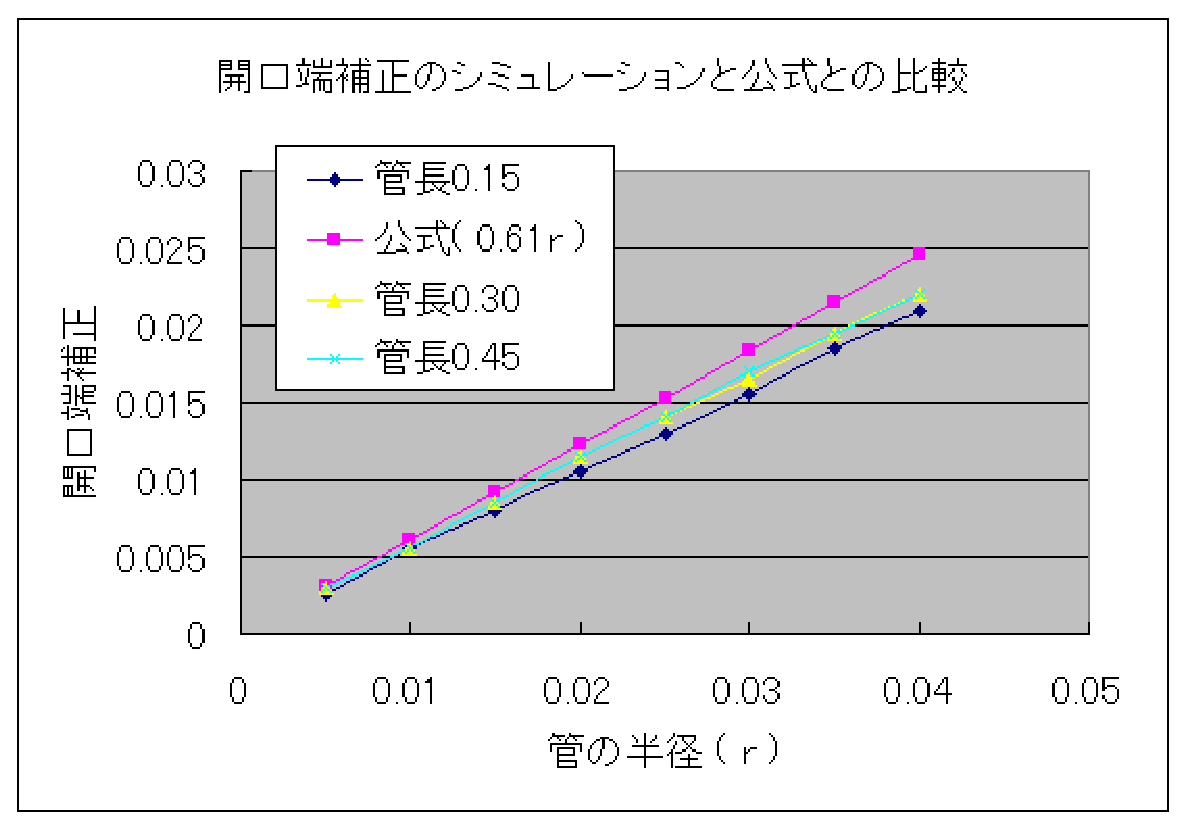
\includegraphics[width=\hsize]{images/compare_open_end_modify.eps}
\caption{axis symmetric region}
\end{center}
\end{figure}

{\bf almost exactly matches the theoretical value with no precision}

The theoretical value of this open end correction is introduced on the \ cite {levy} next page.



\end{document}
